\section{Auswertung}
\label{sec:Auswertung}

%a)
\subsection{Effektiver Widerstand und Abklingdauer} 
Die Zeit und die Amplitude der Spannung sind in Tabelle
\ref{tab1} dargestellt. Um den effektiven Dämpfungswiderstand
zu berechnen, werden die Werte linearisiert. Diese Werte sind in
Tabelle \ref{taba} zu finden. In Abb. \ref{fig:plota}
sind die linearisierten Werte dargestellt. Es wird der
Logarithmus der Spannung gegen die Zeit aufgetragen.
\begin{table}\caption{Der maximale Drehimpuls $L$, der Gesamtspin $S$ und der Gesamtdrehimpuls $J$ ergeben sich zum Landé-Faktor $g_\text{J}$ für die vier verschiedenen Elemente.}
\label{tab1}
\centering
\sisetup{round-mode = places, round-precision=2, round-integer-to-decimal=true}
\begin{tabular}{S[]S[]S[]S[]} 
\toprule
{$L$} & {$S$} & {$J$} & {$g_\text{J}$}\\
\midrule
5.0 & 1.0 & 4.0 & 0.8\\
0.0 & 3.5 & 3.5 & 2.0\\
6.0 & 1.5 & 4.5 & 0.7272727272727273\\
5.0 & 2.5 & 7.5 & 1.3333333333333333\\
\bottomrule
\end{tabular}\end{table}
\begin{table}\caption{Die Länge der Zylinder und die Spannung mit den jeweiligen Zeitenpunkten der Ausschläge.}
\label{taba}
\centering
\sisetup{round-mode = places, round-precision=2, round-integer-to-decimal=true}
\begin{tabular}{S[]S[]S[]S[]S[]} 
\toprule
{$l/ \si{\milli\meter}$} & {$U_1/ \si{\volt}$} & {$t_1/ \si{\micro\second}$} & {$U_2/ \si{\volt}$} & {$t_2/ \si{\micro\second}$}\\
\midrule
120.8 & 1.29 & 0.6 & 0.17 & 88.7\\
102.3 & 1.27 & 0.5 & 0.2 & 76.5\\
80.5 & 1.33 & 0.6 & 0.76 & 59.8\\
40.4 & 1.33 & 0.5 & 1.34 & 30.2\\
31.1 & 1.29 & 0.5 & 1.37 & 23.8\\
\bottomrule
\end{tabular}\end{table}
\begin{figure}
  \centering
  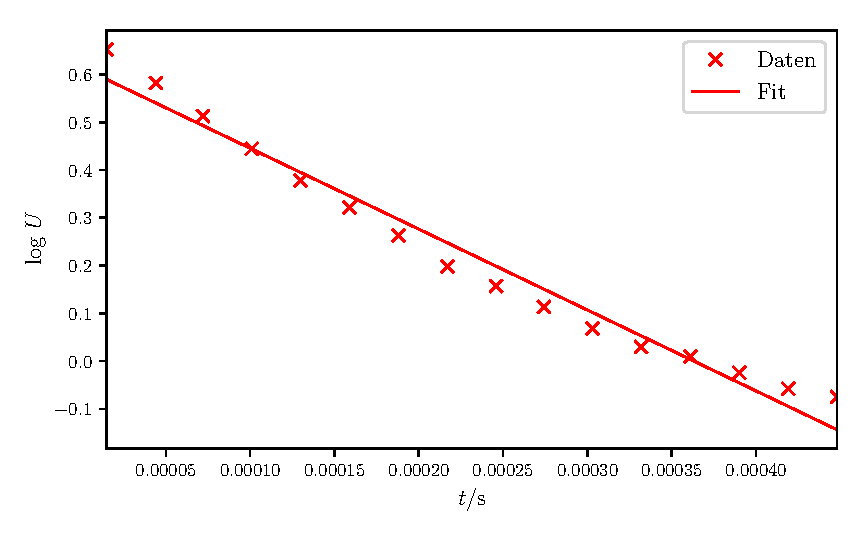
\includegraphics{build/plota.pdf}
  \caption{Die logarithmierte Spannung ist gegen die Zeit aufgetragen.} %Erklären, was die Steigung ist
  \label{fig:plota}
\end{figure}
\noindent Daraus ergibt sich durch \eqref{eqn:reff} %die Steigung???
der effektive Widerstand zu $R_{eff} = \SI{34.2 \pm 1.5}{\ohm}$.
Die Abklingdauer \ref{eqn:t_ex} ist somit $T_{ex} = \SI{0.000590 \pm 0.000026}{\second}$.
%Ist T_ex = 1/R_eff? Hier wurde jetzt dieselbe Gleichung für den experimentalen
%und den theoretischen Wert benutzt.
\newline
Der theoretische effektive Widerstand ist $R_{eff,theo} = \SI{48.1 \pm 0.1}{\ohm}$ %Gleichung angeben
und die Abklingdauer \eqref{eqn:t_ex} $T_{ex,theo} = \SI{0.0004204 \pm 0.0000015}{\second}$. %ex für experimental?

\subsection{Dämpfungswiderstand beim aperiodischen Grenzfall}
%b)
Der Wert für den Dämpfungswiderstand beim aperiodischen Grenzfall
lässt sich ablesen. Er ist $R_{ap} = \SI{3500.0}{\ohm}$.
\newline
Der theoretisch berechnete Wert, der mittels \eqref{eqn:r_ap}
bestimmt wird, ist $R_{ap,theo} = (4390 \pm 9) \si{\ohm}$.

\subsection{Resonanzüberhöhung und Breite der Resonanzkurve}
%c)
Tabelle \ref{tab2} beinhaltet die Spannung der Kondensators
sowie die Abstände der Nulldurchgänge der Kondensatorspannung
und der Erregerspannung zu verschiedenen Frequenzen.
Die Werte zur Berechnung von %?
sind in Tabelle \ref{tabc} aufgelistet.
Die Abbildung \ref{fig:plotc} stellt diese Werte dar.
\begin{table}\caption{Das Verhältnis des magnetischen Feldes durch die Beschleunigungsspannung aufgetragen gegen die Höhe.}
\label{tab2}
\centering
\sisetup{round-mode = places, round-precision=2, round-integer-to-decimal=true}
\begin{tabular}{S[]S[]S[]} 
\toprule
{$B_1 / \si{\henry}$} & {$B_2 / \si{\henry}$} & {$\frac{D}{(L^2 + D^2)} / \si{\per\meter}$}\\
\midrule
0.0 & 0.0 & 0.0\\
3.5649278338607584e-07 & 3.862005153349155e-07 & 0.29289724188430566\\
8.912319584651897e-07 & 8.912319584651897e-07 & 0.5827222842713544\\
1.4259711335443034e-06 & 1.396263401595464e-06 & 0.8665094112549946\\
1.9250610302848096e-06 & 1.8418793808280586e-06 & 1.1414982164090373\\
2.3885016486867084e-06 & 2.3172030920094934e-06 & 1.4052180429996723\\
2.923240823765822e-06 & 2.822234535139767e-06 & 1.6555530006898145\\
3.4223307205063282e-06 & 3.3272659782700412e-06 & 1.8907846756403912\\
\bottomrule
\end{tabular}\end{table}
\begin{table}\caption{Der Anodenstrom und der Kathodenstrom bei einer Beschleunigungsspannung von $U_\text{B} = \SI{25}{\kilo\volt}$ und einer Kathodenspannung $U_\text{K,1} = \SI{500}{\volt}$ und einer Kathodenspannung $U_\text{K,2} = \SI{300}{\volt}$ bei einem Blendenradius von $r_\text{B} = \SI{5}{\milli\meter}$.}
\label{tabc}
\centering
\sisetup{round-mode = places, round-precision=2, round-integer-to-decimal=true}
\begin{tabular}{S[]S[]S[]} 
\toprule
{$I_\text{K} / \si{\milli\ampere}$} & {$I_\text{K,1} / \si{\nano\ampere}$} & {$I_\text{K,2} / \si{\nano\ampere}$}\\
\midrule
1.0 & 2.6 & 2.4\\
0.95 & 2.5 & 2.4\\
0.9 & 2.4 & 2.2\\
0.85 & 2.3 & 2.1\\
0.8 & 2.2 & 2.0\\
0.75 & 2.1 & 1.9\\
0.7 & 1.9 & 1.8\\
0.65 & 1.8 & 1.6\\
0.6 & 1.6 & 1.5\\
0.55 & 1.5 & 1.4\\
0.5 & 1.4 & 1.3\\
0.45 & 1.2 & 1.2\\
0.4 & 1.1 & 1.0\\
0.35 & 0.9 & 0.9\\
0.3 & 0.8 & 0.8\\
0.25 & 0.6 & 0.6\\
0.2 & 0.5 & 0.5\\
0.15 & 0.4 & 0.4\\
0.1 & 0.1 & 0.2\\
0.05 & 0.1 & 0.1\\
\bottomrule
\end{tabular}\end{table}
\begin{figure}
  \centering
  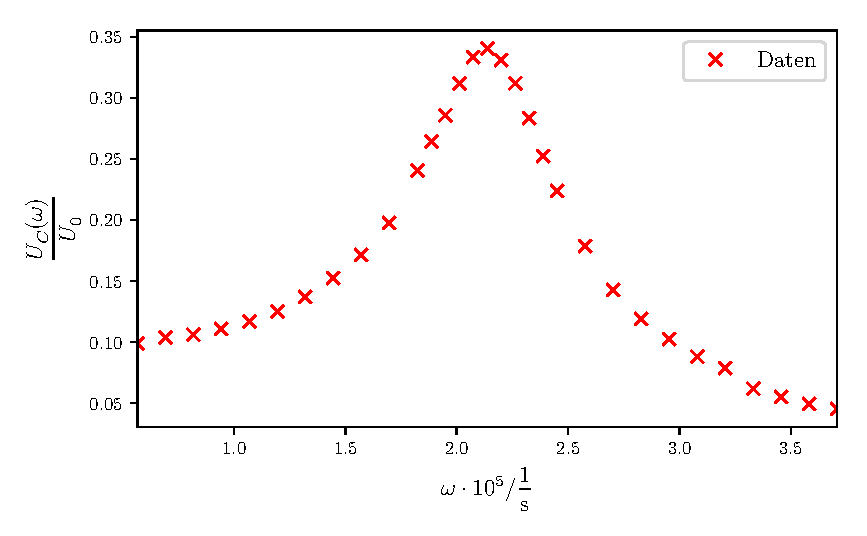
\includegraphics{build/plotc.pdf}
  \caption{Die Amplitude der Kondensatorspannung geteilt durch die Generatorspannung
  ist gegen die Kreisfrequenz aufgetragen. Das Maximum ist die Güte. Es liegt bei der
  Resonanzfrequenz.}
  \label{fig:plotc}
\end{figure}
\noindent Daraus lässt sich der Wert für die Resonanzüberhöhung, bzw. die Güte $q$ entnehmen.
Sie ist nach Gleichung \eqref{eqn:ucmax} das Maximum.
%Die Resonanzfrequenz ist der zugehörige $\omega$-Wert.
Also ergibt sich für die Güte $q = \num{3.40}$.
%und für die Resonanzfrequenz $\omega_{res} = \SI[per-mode=fraction]{213628.30}{\per\second}$.
%omega_+ und omega_- einfügen
Der Breite der Resonanzkurve ist
$\omega_{+} - omega_{-} = \SI[per-mode=fraction]{62831.85}{\per\second}$. %wie?
\newline
Der theoretisch errechnete Wert für die Güte, der mit Gleichung
\eqref{eqn:q} bestimmt werden kann, ist $q_{theo} = \num{4.309 \pm.010}$.
Der mit Gleichung \eqref{eqn:breite} berechnete Wert für die Breite der
Resonanzkurve ist
$\omega_{+,theo} - \omega_{-,theo} = \SI[per-mode=fraction]{5.040(016)e4}{\per\second}$.

\subsection{Resonanzfrequenz} %und omega_1, omega_2?
%d)
Die Abstände der Nulldurchgänge der Kondensatorspannung und
der Erregerspannung sind bereits in Tabelle \ref{tab2}
dargestellt. In Tabelle \ref{tabd} befinden sich die
zur Berechnung von $\omega_{res}$, $\omega_{1}$ und $\omega_{2}$
nötigen Werte, welche auch in Abb. \ref{fig:plotd} gegeneinander
aufgetragen sind. Die Phase wird dabei durch Gleichung \eqref{eqn:phi}
bestimmt.
\begin{table}\caption{Laufzeiten und Spannungen der reflektierten Impulse bei dem Modell des Auges.}
\label{tabd}
\centering
\sisetup{round-mode = places, round-precision=2, round-integer-to-decimal=true}
\begin{tabular}{S[]S[]} 
\toprule
{$t_1/ \si{\micro\second}$} & {$U_1/ \si{\volt}$}\\
\midrule
1.0 & 1.38\\
11.7 & 1.0\\
16.1 & 1.25\\
22.9 & 0.95\\
72.2 & 0.4\\
\bottomrule
\end{tabular}\end{table}
\begin{figure}
  \centering
  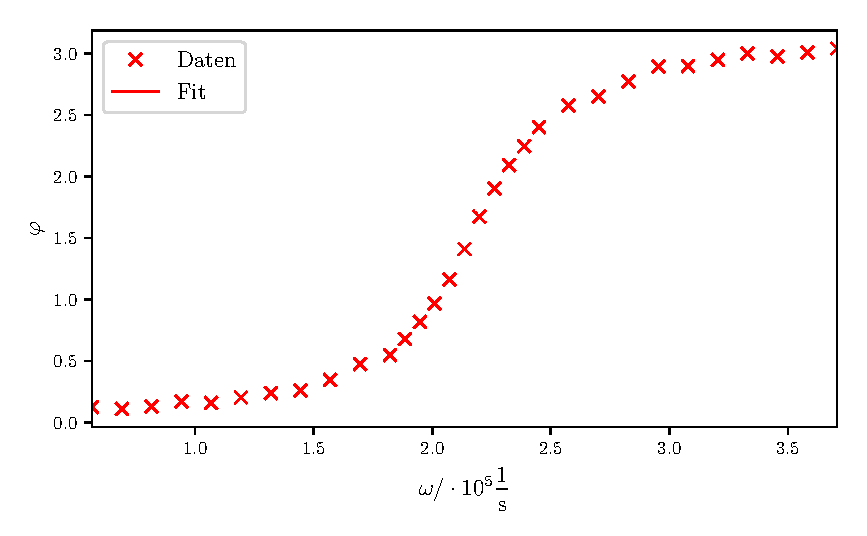
\includegraphics{build/plotd.pdf}
  \caption{Die Phasenverschiebung der Kondensatorspannung und der
  Generatorspannung ist gegen die Kreisfrequenz aufgetragen.} %Erklären, was die Steigung ist
  \label{fig:plotd}
\end{figure}
\noindent Aus Abbildung \ref{fig:plotd} kann man die gesuchten Werte entnehmen. %wie?
Die Resonanzfrequenz ist $\omega_{res} = \SI[per-mode=fraction]{213628.30}{\per\second}$.
$\omega_{1}$ und $\omega_{2}$ haben die Werte
$\omega_{1} = \SI[per-mode=fraction]{182212.37}{\per\second}$ und
$\omega_{2} = \SI[per-mode=fraction]{245044.23}{\per\second}$.
\newline
Die Resonanzfrequenz lässt sich in der Theorie durch 
Gleichung \eqref{eqn:omega_res} bestimmen.
Der Wert für diese ist $\omega_{res,theo} = \SI[per-mode=fraction]{2.142(004)e5}{\per\second}$.
Für die Frequenzen $\omega_{1,theo}$ und $\omega_{2,theo}$ ergibt sich
mittels Gleichung \eqref{eqn:omega_12}:
$\omega_{1,theo} = \SI[per-mode=fraction]{1.934(004)e5}{\per\second}$ und
$\omega_{2,theo} = \SI[per-mode=fraction]{2.438(005)e5}{\per\second}$.
